
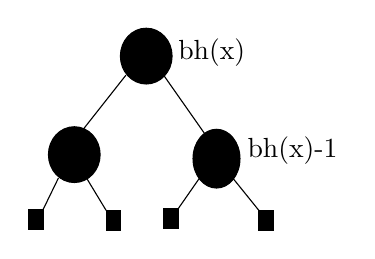
\begin{tikzpicture}[x=0.4pt,y=0.4pt,yscale=-1,xscale=1]
%uncomment if require: \path (0,706); %set diagram left start at 0, and has height of 706

\draw  [fill={rgb, 255:red, 0; green, 0; blue, 0 }  ,fill opacity=1 ]  (242.83, 180.82) circle [x radius= 23.33, y radius= 25.18]  ;
\draw  [fill={rgb, 255:red, 0; green, 0; blue, 0}  ,fill opacity=1 ]  (306.3, 273.47) circle [x radius= 21.2, y radius= 26.53]  ;
\draw  [fill={rgb, 255:red, 0; green, 0; blue, 0 }  ,fill opacity=1 ]  (136.22, 319.65) rectangle (149.54, 337.61)   ;
\draw    (149.54,319.65) -- (163.5,291) ;


\draw    (258.5,198) -- (298.5,255) ;


\draw  [fill={rgb, 255:red, 0; green, 0; blue, 0 }  ,fill opacity=1 ]  (177.83, 269.82) circle [x radius= 23.33, y radius= 25.18]  ;
\draw    (183.5,250) -- (224.5,198) ;


\draw    (189.5,292) -- (206.62,320.26) ;


\draw    (321,291) -- (344.62,320.26) ;


\draw    (271.83,318.48) -- (292.26,289.13) ;


\draw  [fill={rgb, 255:red, 0; green, 0; blue, 0 }  ,fill opacity=1 ]  (206.62, 320.26) rectangle (219.94, 338.22)   ;
\draw  [fill={rgb, 255:red, 0; green, 0; blue, 0 }  ,fill opacity=1 ]  (258.5, 318.48) rectangle (271.83, 336.44)   ;
\draw  [fill={rgb, 255:red, 0; green, 0; blue, 0 }  ,fill opacity=1 ]  (344.62, 320.26) rectangle (357.94, 338.22)   ;

\draw (302,178) node  [align=left] {bh(x)};
\draw (375,266) node  [align=left] {bh(x)-1};


\end{tikzpicture}